\chapter{Diseño de firmware}
En este capítulo se describen todas las etapas necesarias para desarrollar un sistema de adquisición de datos capaz de generar una imagen. Estas etapas abarcan la caracterización de resistencias, multiplexores y una fotorresistencia, además del diseño de una PCB para una matriz de fototransistores. Finalmente, se presenta el diseño digital implementado para adquirir una imagen. Todos los diseños fueron implementados en la tarjeta Basys 3 de Digilent, que cuenta con una FPGA Artix-7 (XC7A35T-1CPG236C).

\section{Caracterización de resistencias}
En esta etapa, se realizó la caracterización de cuatro resistencias utilizando un circuito divisor de voltaje (Figura \ref{fig:divisor2}). En este circuito, $R_{test}$ simula la resistencia de un pixel de un arreglo de microbolómetros, mientras que $R_{ref}$ emula un circuito de lectura. Trabajar con resistencias de valores conocidos permite verificar con mayor precisión si los resultados experimentales coinciden con los teóricos. 


            \begin{figure}[hbtp]
                \centering
                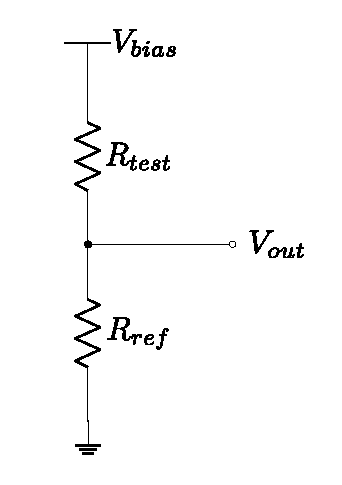
\includegraphics[width=0.3\textwidth]{divisor2}
                \caption{Divisor de voltaje como microbolómetro y circuito de lectura}
                \label{fig:divisor2}
            \end{figure} 


Para determinar cuál es el valor más adecuado de $R_{ref}$ para cualquier $R_{test}$ y el voltaje de polarización del circuito, se llevó a cabo una simulación de dos circuitos en LTSpice. En ambos circuitos, se realizó un barrido de $R_{test}$ desde $1k\Omega$ hasta $10k\Omega$, con incrementos de $1k\Omega$, con el fin de imitar un microbolómetro bajo la influencia de luz y un barrido de la fuente de voltaje $V_{1}$ de $0V$ a $3.3V$ en incrementos de $0.1V$. La única diferencia entre los circuitos fue el valor de $R_{ref}$: en uno de ellos, $R_{ref}$ se fijó en $1k\Omega$, mientras que en el otro se estableció en $10k\Omega$. Esta comparación permitió evaluar cómo afectaba el valor de $R_{ref}$ en la respuesta del sistema ante distintos valores de $R_{test}$, facilitando la selección del valor más adecuado para optimizar la lectura del circuito.

            \begin{figure}[hbtp]
                \centering
                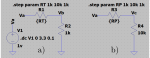
\includegraphics[width=0.8\textwidth]{cto_ltspice}
                \caption{Divisores de voltaje para la elección de $R_{ref}$}
                \label{fig:cto_ltspice}
            \end{figure}


En las Figuras \ref{fig:graph_1k} y \ref{fig:graph_10k} se presentan los resultados de los barridos de $R_{test}$.


Supongase que estos resultados son de un microbolómetro cuya resistencia no se puede medir directamente, salvo a través del circuito de lectura, $R_{ref}$, y despejando $R_{test}$ de la ecuación del divisor de voltaje. Al polarizar el circuito divisor con voltajes muy bajos, resulta imposible identificar con precisión la resistencia del detector. No obstante, al polarizar a partir de $2.7V$, se vuelve más fácil determinar el valor de $R_{test}$.

            \begin{figure}[hbtp]
                \centering
                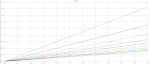
\includegraphics[width=1\textwidth]{graph_1k}
                \caption{Gráficas de voltaje de $R_{ref} = 1k\Omega$ con barrido en $R_{test}$}
                \label{fig:graph_1k}
            \end{figure}
            
Sin embargo, es importante señalar que la influencia de $R_{ref}$ también juega un papel crucial. En la Figura \ref{fig:graph_1k}, con $R_{ref} = 1k\Omega$, se observa que, para valores altos de $R_{test}$, resulta difícil conocer con precisión la resistencia del detector, siendo únicamente posible identificarla para valores menores a $6k\Omega$. En contraste, en la Figura \ref{fig:graph_10k}, donde $R_{ref} = 10k\Omega$, las curvas para cualquier $R_{test}$ no se empalman y es más sencillo identificar la resistencia del detector, esto llevó a optar por un valor de $R_{ref} = 10k\Omega$ para la caracterización de resistencias.
 
            \begin{figure}[hbtp]
                \centering
                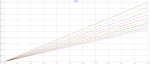
\includegraphics[width=1\textwidth]{graph_10k}
                \caption{Gráficas de voltaje de $R_{ref} = 10k\Omega$ con barrido en $R_{test}$}
                \label{fig:graph_10k}
            \end{figure}

Finalmente, se seleccionaron como $R_{test}$ las resistencias de $1k\Omega$, $3.3k\Omega$, $5.6k\Omega$ y $10k\Omega$ con el objetivo de simular el comportamiento de un microbolómetro en función de la cantidad de luz recibida y para proporcionar una mayor variedad en los resultados.


Una vez realizadas las simulaciones y seleccionados los valores de $R_{test}$ y $R_{ref}$, se procedió al diseño digital en FPGA para la caracterización de resistencias. Este diseño incluyó la implementación de un barrido de voltaje, realizado mediante una memoria ROM y un convertidor D/A, cuyos voltajes se encargan de polarizar el circuito divisor de voltaje. La lectura y conversión de la caída de voltaje en $R_{ref}$ fue llevado a cabo empleando un convertidor A/D, estas conversiones fueron transmitidas a MATLAB a través del protocolo RS232 para su posterior procesamiento.


El diseño digital para la caracterización de resistencias se compone de varios módulos interconectados que permiten la adquisición de datos.
Estos módulos son:


\begin{itemize}
    \item Memoria ROM (rom volts): Contiene valores en binario correspondientes a voltajes de $0V$ a $3V$, con incrementos de $0.1V$. La salida de la memoria ROM está conectada al módulo de escritura del convertidor D/A.

    \item Escritura del DAC (spi write dac): Convierte y transmite los voltajes guardados en la memoria ROM al circuito divisor de voltaje, permitiendo la polarización del circuito.

    \item Escritura y lectura del ADC (spi write read adc): Lee y convierte la caída de voltaje en $R_{ref}$. Los valores obtenidos son almacenados en una memoria RAM.

    \item Memoria RAM (ram volts): Almacena los voltajes convertidos por el ADC, y su función principal es conservar el valor de la resistencia del microbolómetro ante posibles cambios en la iluminación.
    
    La palabra de 12 bits obtenida de la RAM se divide en dos partes: una de 8 bits (bits menos significativos) y otra de 4 bits (bits más significativos). La parte de 4 bits se concatena con cuatro ceros, formando así dos palabras de 8 bits, que luego se conectan a un multiplexor.
    

    \item Multiplexor (mux ch): Selecciona cuál de las dos palabras de 8 bits almacenadas en la RAM será transmitida a través del módulo UART.


    \item Transmisión (uart tx): Envía los datos guardados en la RAM y organizados por el multiplexor hacia MATLAB para su procesamiento.

    \item Contadores: Se utilizan dos contadores con selector, uno para la memoria ROM (counter volts) y otro para la memoria RAM (counter address). Ambos son empleados para direccionar los datos de manera adecuada.

    \item Máquina de estados (fsm dac adc tx): Es el módulo más importante, compuesto por 17 estados, se encarga de habilitar y coordinar el funcionamiento de todos los módulos anteriormente mencionados. A continuación, se explica la función de cada uno de los estados.
    \begin{enumerate}
     \item s0: La máquina de estados espera una señal de activación, la cual proviene de un push button.
     \item s1: Una vez activada, se habilita la escritura del DAC para iniciar el proceso de conversión de voltaje.
     \item s2: El DAC se deshabilita, y el sistema permanece en este estado mientras la bandera \textit{end of DAC} (eodac) sea cero. Cuando la bandera cambia a 1, indica que el DAC ha completado su conversión.
     \item s3 y s4: Estados de guarda que aseguran que el circuito divisor de voltaje esté correctamente polarizado.
     \item s5: Se activa el ADC para iniciar la lectura del voltaje de $R_{ref}$.
     \item s6: El ADC se desactiva, y el sistema permanece en este estado mientras la bandera \textit{end of ADC} (eoadc) sea cero. Cuando cambia a 1, significa que el ADC ha terminado su conversión.
     \item s7: Se habilita la RAM y se almacena la conversión realizada por el ADC.
     \item s8: La RAM se deshabilita, y se incrementan los contadores de la ROM y la RAM.
     \item s9: El sistema mantiene el valor de los contadores y verifica si el contador de la RAM ha llegado a 31. Si es cierto, pasa al estado s10; si no, vuelve al estado s1.
     \item s10: Se reinician los contadores de la ROM y la RAM.
     \item s11: Se habilita el módulo de transmisión para comenzar a enviar datos.
     \item s12: La transmisión se deshabilita, y el sistema permanece en este estado hasta que la bandera \textit{end of transmission} (eotx) indique que se han enviado los 8 bits más significativos de la salida de la RAM. 
     \item s13: Se habilita nuevamente la transmisión, y el selector del multiplexor se pone a 1 para enviar los 8 bits menos significativos de la salida de la RAM.
     \item s14: La transmisión se desactiva, y el sistema espera hasta que se haya terminado de transmitir los bits menos significativos.
     \item s15: El contador de la RAM se incrementa para enviar el siguiente conjunto de datos.
     \item s16: El sistema mantiene el valor del contador de la RAM y verifica si ha llegado a 31. Si es cierto, se regresa al estado s0 para repetir el proceso; de lo contrario, se vuelve al estado s11 para continuar la transmisión.           
    \end{enumerate}
\end{itemize}

Los códigos de los módulos descritos anteriormente se encuentran en el \textbf{Apéndice A}, sección \textbf{A.2.3.5}.


\section{Caracterización de multiplexores}
Cuando se quiere trabajar con una matriz de $m \times n$ detectores, se deben emplear dos multiplexores: uno para direccionar las columnas y otro para las filas de la matriz. En este trabajo se utilizaron los multiplexores 74HC4051, cada uno con 8 entradas/salidas (Yn), una entrada/salida común (Z), tres entradas digitales de selección (S0-S2) y un pin de habilitación (E), activo en bajo. Estos multiplexores pueden alimentarse con un voltaje en el rango de $-5V$ a $+5V$.


Al utilizar una matriz de detectores, es esencial comprender cómo los multiplexores afectan el circuito, ya que, al estar conectados a la matriz, influyen en el valor del voltaje que debe caer sobre el circuito de lectura. Para evaluar este impacto, se emplearon las cuatro resistencias seleccionadas como $R_{test}$, organizándolas en forma de matriz. Los multiplexores fueron alimentados con $3.3V$ mediante la tarjeta Basys 3, y se utilizaron los mismos códigos que en la caracterización de resistencias. No fue necesario desarrollar código adicional para controlar los multiplexores, ya que estos se operaron manualmente durante las pruebas.


A continuación, se presenta la tabla de verdad del 74HC4051, que muestra cómo debe ser controlado.
            \begin{table}[htbp]
                \caption{Tabla de verdad de multiplexor 74HC4051.}
                \begin{center}
                    \resizebox{0.4\linewidth}{!}{ 
                    \begin{NiceTabular}{|l l l l|l|}
                        \CodeBefore
                        \Body
                        \hline
                        \multicolumn{4}{ |c| }{Inputs}\\
                        $\overline{E}$ & S2 & S1 & S0 & Channel ON\\
                        \hline
                        L & L & L & L & Y0 to Z\\
                        L & L & L & H & Y1 to Z\\
                        L & L & H & L & Y2 to Z\\
                        L & L & H & H & Y3 to Z\\
                        L & H & L & L & Y4 to Z\\
                        L & H & L & H & Y5 to Z\\
                        L & H & H & L & Y6 to Z\\
                        L & H & H & H & Y7 to Z\\
                        H & X & X & X & switches off\\                                                                        
                        \hline
                    \end{NiceTabular}
                    }
                \label{tab:true_table_mux}
                \end{center}
            \end{table}


\section{Caracterización de fotorresistencia}
Se utilizó una fotorresistencia para tener una referencia clara de cómo sería trabajar con un microbolómetro real, debido a que ambos detectores comparten un comportamiento similar: en ausencia de luz, su resistencia aumenta, mientras que bajo iluminación, disminuye. En este caso, se empleó la fotorresistencia GL5537, que presenta una resistencia de $2M\Omega$ en oscuridad y un rango de $20K\Omega$ a $30K\Omega$ bajo luz, con un tiempo de respuesta de 20 ms.

Primero, la fotorresistencia fue caracterizada bajo la iluminación de las lámparas de un salón. Posteriormente, se realizaron pruebas en condiciones controladas dentro de una caja oscura, midiendo su resistencia en ausencia de luz. Para simular diferentes niveles de iluminación, se incorporó un LED de 3W, cuya intensidad fue regulada mediante un PWM con cuatro ciclos de trabajo: $25\%$, $50\%$, $75\%$ y $100\%$.

El diseño digital empleado para esta caracterización es similar al utilizado en la caracterización de resistencias, con la diferencia de que se agregó un módulo PWM para controlar la iluminación y observar la respuesta de la fotorresistencia. 



\section{Sistema de adquisición de datos}
En esta etapa final, se desarrolló una PCB para una matriz de $8\times 8$ fototransistores, diseñada en Altium Designer, con el propósito de generar una imagen. En esta sección, se explicará primero el proceso de diseño de la matriz y, posteriormente, el diseño digital. Varios de los módulos implementados en etapas anteriores fueron reutilizados, junto con la incorporación de nuevos módulos para la obtención de imágenes.

\subsection{Diseño de PCB}
Antes de proceder con el diseño de la PCB, se realizó una búsqueda exhaustiva de detectores que pudieran ser adecuados para generar una imagen. Tras analizar varias opciones, se determinó que el fototransistor ALS-PT19-315C, un detector de luz visible, era el más apropiado, debido a su tiempo de respuesta. Además este sensor ha sido utilizado exitosamente en proyectos similares, lo que garantiza su fiabilidad en aplicaciones de imágenes. Otros factores que influyeron en su selección fueron su precio accesible y su amplia disponibilidad en stock. Adicionalmente, se decidió implementar una matriz de $8\times 8$ fototransistores, ya que este número coincide con las entradas/salidas disponibles en los multiplexores seleccionados. Con esta información se procedió al desarrollo de la PCB. 


La creación de la librería de esquemáticos fue el primer paso en el diseño de la PCB. En este caso, los únicos componentes que se incorporaron fueron los headers de $1\times 8$ y el fototransistor ALS-PT19-315C (Figura \ref{fig:sch_lib}), dado que estos elementos se emplean repetidamente en la matriz de $8\times 8$, no fue necesario agregar más componentes a la librería.


            \begin{figure}[hbtp]
                \centering
                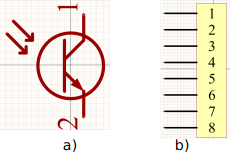
\includegraphics[width=0.5\textwidth]{sch_lib}
                \caption{Componentes de librería de esquemáticos: a) fototransistor, b) pines de $1\times 8$.}
                \label{fig:sch_lib}
            \end{figure}

El segundo paso fue realizar el esquemático de la matriz, el cual se muestra en la Figura \ref{fig:sch_matrix}. En esta etapa, se realizaron las conexiones entre los componentes, asegurando que cada fototransistor y header estuvieran correctamente vinculados según el diseño de la matriz. Además, en este paso también se asignaron los nombres a las pistas de la PCB, lo que facilita la organización y el enrutamiento de las señales. Este proceso es crucial para asegurar que todos los componentes interactúen correctamente.
            \begin{figure}[hbtp]
                \centering
                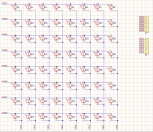
\includegraphics[width=0.8\textwidth]{sch_matrix}
                \caption{Esquemático de matriz de fototransistores.}
                \label{fig:sch_matrix}
            \end{figure}
            
El siguiente paso fue la generación de los pads de los componentes. Los pads en una PCB son áreas de contacto metálico diseñadas para permitir la conexión eléctrica y mecánica entre los componentes electrónicos y la propia placa. Para garantizar que los pads fueran precisos y compatibles con los componentes utilizados, se revisó el datasheet de cada uno. En este caso, los fototransistores utilizados son de tipo SMD (Surface Mounting Device), lo que requiere pads específicos para montaje superficial, mientras que los headers son THT (Through-Hole Technology), lo que implica la necesidad de pads con perforaciones para su montaje.


Los pads del fototransistor se muestran en la siguiente imagen.

            \begin{figure}[hbtp]
                \centering
                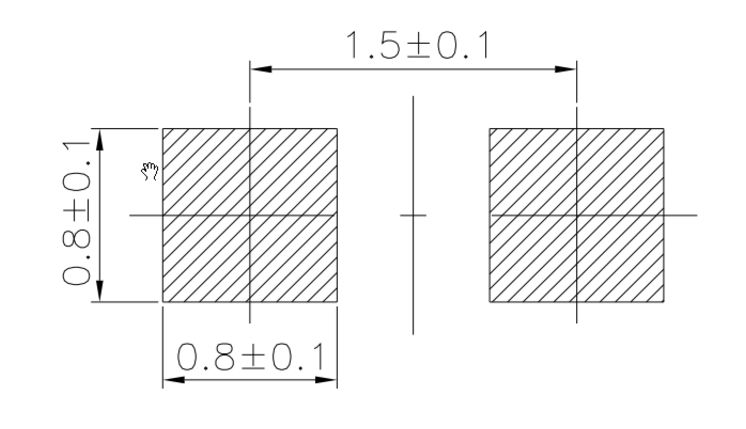
\includegraphics[width=0.5\textwidth]{pad_als}
                \caption{Pads de fototransistor ALS-PT19-315C.}
                \label{fig:pad_als}
            \end{figure}

Las dimensiones de los pads, de acuerdo con el datasheet del fototransistor, están especificados en milímetros. En Altium Designer, se definió un tamaño de pad de $0.9 \times 0.9$ mm con un pitch (la distancia entre los centros de los pads) de 1.6 mm (Figura \ref{fig:pad_altium_als}). Es importante optar por la mayor dimensión indicada en el datasheet, tanto por seguridad ante posibles variaciones en el tamaño del componente como para asegurar una correcta distribución de la soldadura durante el montaje del componente.

            \begin{figure}[hbtp]
                \centering
                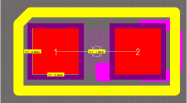
\includegraphics[width=0.65\textwidth]{pad_altium_als}
                \caption{Pads de fototransistor ALS-PT19-315C realizados en Altium Designer.}
                \label{fig:pad_altium_als}
            \end{figure}

Los pads para los headers de $1\times 8$ siguen dimensiones estandarizadas, lo que facilita su integración en diversos diseños de PCBs. El tamaño de los pads es de 1.2 mm, con un pitch de 2.54 mm (Figura \ref {fig:pad_altium_hdr}), estándar para la mayoría de los conectores de este tipo. Además, los headers $1\times 8$ tienen una longitud aproximada de 20 mm y un ancho de 3 mm.

            \begin{figure}[hbtp]
                \centering
                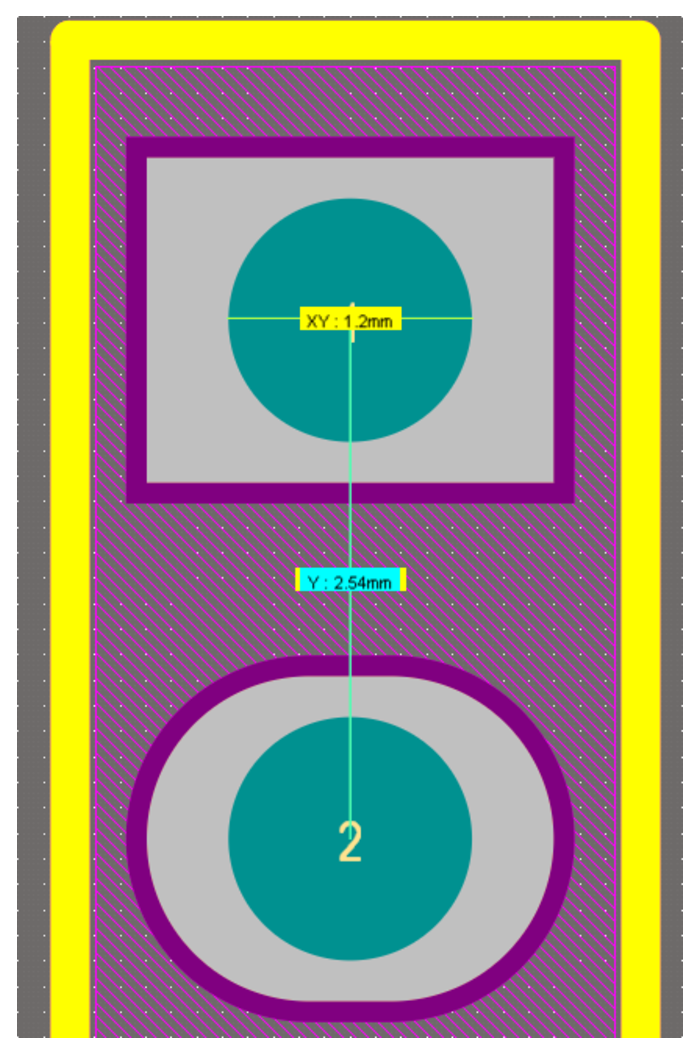
\includegraphics[width=0.4\textwidth]{pad_altium_hdr}
                \caption{Pads de header $1 \times 8$ realizados en Altium Designer.}
                \label{fig:pad_altium_hdr}
            \end{figure}

Finalmente, se procedió a dar forma a la PCB, organizando los componentes según las necesidades del diseño. Se optó por colocar cada fototransistor en un ángulo de 45°, formando una matriz cuadrada que optimiza el espacio y garantiza una disposición uniforme de los detectores. Para el diseño de la tarjeta, se establecieron varias reglas clave, definidas por el fabricante: el clearance (espacio entre pistas) fue de 2.54 mm, el ancho de las pistas de 0.3 mm, los agujeros con un diámetro mínimo de 0.254 mm y un máximo de 5 mm, y las vías con un diámetro externo de 0.6 mm y un diámetro interno de 0.3 mm. 


Tras cotizar con varios proveedores, JLCPCB resultó ser la opción más conveniente en términos de precio y calidad. La PCB diseñada fue de 2 capas, con dimensiones de 40x40 mm, un grosor de 1.6 mm y fabricada en material FR-4.


En la Figura \ref{fig:pcb_matrix}, se puede apreciar el diseño final de la PCB. Nótese que hay dos colores distintos en las pistas: las pistas de color rojo corresponden a las que pasan por la parte superior de la tarjeta, mientras que las de color azul representan las que pasan por la parte inferior. Esta distribución de las pistas en ambas caras de la tarjeta es la razón por la cual la PCB tiene 2 capas.


            \begin{figure}[hbtp]
                \centering
                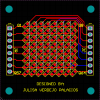
\includegraphics[width=0.6\textwidth]{pcb_matrix}
                \caption{Diseño de PCB para una matriz de fototransistores.}
                \label{fig:pcb_matrix}
            \end{figure}

\subsection{Diseño digital}
El fototransistor ALS-PT19-315C es un sensor diseñado para detectar luz visible y puede ser alimentado con un voltaje que varía entre $2.5V$ y $5V$. Presenta una corriente en oscuridad de 0.1$\mu$A. Además, cuenta con un rise time de 0.11 ms y un fall time de 0.22 ms, lo que le permite responder rápidamente a los cambios en la intensidad de la luz. En la siguiente tabla se muestra un resumen de los parámetros mencionados.

            \begin{table}[htbp]
                \caption{Parámetros del fototransistor ALS-PT19-315C}
                \begin{center}
                    \resizebox{0.8\linewidth}{!}{ 
                    \begin{NiceTabular}{|c|c|c|c|c|c| }
                        \CodeBefore
                        \Body
                        \hline
                        \textbf{Parameter} & \textbf{Symbol} & \textbf{Min} & \textbf{Typ} & \textbf{Max} & \textbf{Unit}\\
                        \hline
                        Supply voltage & $V_{CC}$ & 2.5 & --- & 5 & V\\
                        Dark current & $I_{CEO}$ & --- & --- & 0.1 & $\mu$A\\
                        Rise time & $t_{r}$ & --- & 0.11 & --- & ms\\
                        Fall time & $t_{f}$ & --- & 0.22 & --- & ms \\
                        \hline
                    \end{NiceTabular}
                    }
                \label{tab:als_param}
                \end{center}
            \end{table}

Dadas las especificaciones anteriores, se optó por polarizarlo con los $3.3V$ proporcionados por la tarjeta Basys 3, lo que hizo innecesario el uso del DAC en el proceso de adquisición de imágenes.


En el diseño digital, se reutilizaron varios módulos previamente implementados, como los módulos de escritura y lectura del SPI, la transmisión por UART, la memoria RAM, un multiplexor, el debouncer, y un contador para direccionar la RAM. Además, se incorporaron dos contadores de carrera libre de 3 bits: uno para direccionar las filas y otro para las columnas de la matriz de fototransistores, junto con un contador descendente que permite estabilizar el circuito de lectura. Finalmente, se diseñó una máquina de estados específica para coordinar y controlar el proceso de obtención de imágenes.


La máquina de estados diseñada consta de 18 estados, a continuación, se explicará la función de cada uno de ellos.

\begin{itemize}
\item s0: Espera una señal de habilitación, la cual proviene del módulo debouncer para iniciar la máquina de estados.
\item s1: Habilita el contador ascendente y espera a que este llegue a cero.
\item s2 y s3: Estados de guarda.
\item s4: Habilitación del módulo SPI para controlar al ADC.
\item s5: Deshabilita el módulo SPI y permanece en este estado hasta que la conversión finalice.
\item s6: Habilita la memoria RAM para almacenar la caída de voltaje del circuito de lectura, leída y convertida por el ADC.
\item s7: Deshabilita la memoria RAM y habilita el contador de las columnas.
\item s8: Verifica si el contador de las columnas ha llegado a cero. Si es así, pasa al estado s9; de lo contrario, regresa a s1 y repite el ciclo hasta que se cumpla la condición.
\item s9: Activa el contador de las filas.
\item s10: Deshabilita el contador de las filas y verifica si ha llegado a cero. Si es así, pasa al estado s11; de lo contrario, regresa a s1 y repite el ciclo hasta que se cumpla la condición. 
\item s11: Activa la transmisión.
\item s12: Desactiva la transmisión y espera a que esta termine.
\item s13: Cambia el selector del multiplexor a 1.
\item s14: Habilita nuevamente la transmisión.
\item s15: Deshabilita la transmisión y, cuando la bandera eotx sea igual a 1 pasa al estado s16.
\item s16: Cambia el selector del multiplexor a 0 y habilita el contador que direcciona a la memoria RAM para transmitir la siguiente conversión del ADC.
\item s17: Deshabilita el contador de direcciones y verifica si ha llegado a cero. Si es así, regresa al estado s0; de lo contrario, vuelve al estado s11 para realizar una nueva transmisión de datos.
\end{itemize}
